\documentclass[10pt]{article}
\usepackage[a4paper,margin=18mm]{geometry}
\usepackage{amsmath,amssymb,booktabs,array,enumitem,longtable}
\usepackage[T1]{fontenc}\usepackage{lmodern}
\usepackage{tikz}\usetikzlibrary{shapes.gates.logic.US,positioning,arrows.meta,patterns,calc}
\usepackage[hidelinks]{hyperref}
\setlength{\parindent}{0pt}\setlength{\parskip}{4pt}\setlength{\emergencystretch}{2em}
\newcommand{\VDD}{V_{DD}}
\newcommand{\mos}[4]{\begin{scope}[shift={(#1,#2)}]
\draw (0,.24)--(0,-.24);\draw (0,.20)--(.25,.20)--(.25,.5);
\draw (0,-.20)--(.25,-.20)--(.25,-.5);\draw (-.16,.23)--(-.16,-.23);
\ifnum#4=1\draw (-.26,0) circle (.06);\draw (-.75,0)--(-.32,0);\else\draw (-.75,0)--(-.16,0);\fi
\node[anchor=east,font=\scriptsize] at (-.76,0) {$#3$};\end{scope}}
\newcommand{\ground}[2]{\draw (#1,#2)--(#1,{#2-.12});\draw ({#1-.17},{#2-.12})--({#1+.17},{#2-.12});\draw ({#1-.11},{#2-.20})--({#1+.11},{#2-.20});}
\newcommand{\rail}[3]{\draw (#1,#2)--(#1,{#2+.14});\node[above,font=\scriptsize] at (#1,{#2+.14}) {$#3$};}
\newcommand{\hmos}[4]{\begin{scope}[shift={(#1,#2)}]
\draw(-.24,0)--(.24,0);\draw(-.2,0)--(-.2,-.25)--(-.5,-.25);\draw(.2,0)--(.2,-.25)--(.5,-.25);
\draw(-.23,.16)--(.23,.16);
\ifnum#4=1\draw(0,.26)circle(.06);\draw(0,.32)--(0,.75);\else\draw(0,.16)--(0,.75);\fi
\node[below,font=\scriptsize]at(0,-.32){#3};\end{scope}}
\newcommand{\qheading}[1]{\par\medskip\textbf{#1}\par}
\begin{document}
\begin{center}{\Large\bfseries EE332 Introduction to VLSI---Midterm}\\Spring 2008\end{center}
\small Editable reconstruction of original pages 1-1 and 1-2. Study ink is excluded. The first four printed allocations total 90 points; Q5 is printed ``10\%'' and is retained that way.\normalsize
\qheading{1. (40 points) Answer the following problems.}
\begin{enumerate}[label=(\alph*),leftmargin=7mm]
\item What is antenna effect? (4 points)
\item What is channel length modulation effect? (4 points)
\item Draw a CMOS transistor-level schematic realizing $f=\overline{xy+(u+v)w}$. (6 points)
\item List four properties of static CMOS logic. (4 points)
\item List two latchup prevention approaches. (4 points)
\item Draw a CMOS inverter and label the drain and source of the PMOS and NMOS transistors. (4 points)
\item Define the low and high noise margins using the voltage transfer curve of a CMOS inverter. (4 points)
\item List two possible approaches for alleviating the effect of crosstalk on two neighboring parallel interconnects. (4 points)
\item List the three major components of the load capacitance of a CMOS logic gate. (6 points)
\end{enumerate}
\qheading{2. (20 points)} Figure 1(a) depicts a CMOS logic circuit. Assume that the delay of the inverter is 1 delay unit, the inverter size is $W_p/L_p=2\,\mu\mathrm{m}/0.18\,\mu\mathrm{m}$ and $W_n/L_n=1\,\mu\mathrm{m}/0.18\,\mu\mathrm{m}$, and its input capacitance is $C_i$. Also, assume that the size of each NMOS and PMOS transistor of all the other gates is the same as that of the inverter.
\begin{enumerate}[label=(\alph*),leftmargin=7mm]
\item Determine the delay of each gate in terms of delay unit (neglect the diffusion and wire capacitance). (10 points)
\item Assume that a dual-$V_t$ process can be used to implement the CMOS circuit. Draw the transistor schematic diagram in terms of the symbols shown in Fig. 1(b) such that leakage power is minimal without sacrificing the speed of the CMOS circuit. (10 points)
\end{enumerate}
\begin{center}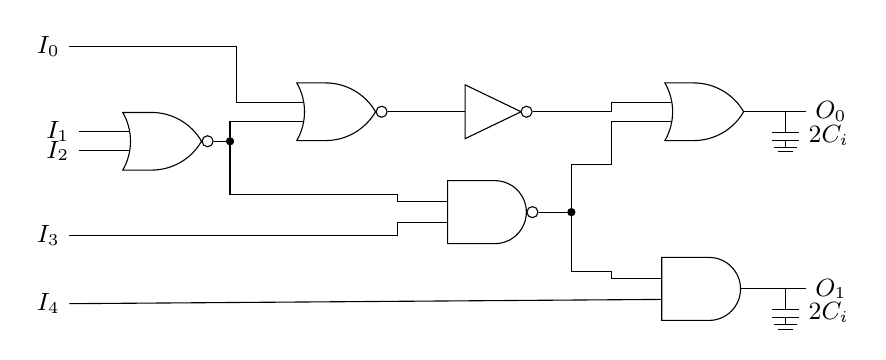
\begin{tikzpicture}[x=.85cm,y=.75cm,font=\small]
\node[nor gate US,draw,logic gate inputs=nn,minimum width=1cm](a)at(1.3,4){};
\node[nor gate US,draw,logic gate inputs=nn,minimum width=1cm](b)at(3.9,4.5){};\node[not gate US,draw,minimum width=.8cm](c)at(6.2,4.5){};
\node[or gate US,draw,logic gate inputs=nn,minimum width=1cm](o)at(9.4,4.5){};
\draw(a.input 1)--++(-.75,0)node[left]{$I_1$};\draw(a.input 2)--++(-.75,0)node[left]{$I_2$};\draw(0,5.6)node[left]{$I_0$}--(2.5,5.6)|-(b.input 1);
\draw(a.output)--(2.4,4)|-(b.input 2);\fill(2.4,4)circle(1.5pt);\draw(b.output)--(c.input);\draw(c.output)--(8.1,4.5)|-(o.input 1);
\node[nand gate US,draw,logic gate inputs=nn,minimum width=1cm](d)at(6.2,2.8){};\node[and gate US,draw,logic gate inputs=nn,minimum width=1cm](g)at(9.4,1.5){};
\draw(2.4,4)--(2.4,3.1)--(4.9,3.1)|-(d.input 1);\draw(0,2.4)node[left]{$I_3$}--(4.9,2.4)|-(d.input 2);
\draw(d.output)--(7.5,2.8)--(7.5,3.6)--(8.1,3.6)|-(o.input 2);\fill(7.5,2.8)circle(1.5pt);
\draw(7.5,2.8)--(7.5,1.8)--(8.1,1.8)|-(g.input 1);\draw(g.input 2)--(0,1.25)node[left]{$I_4$};
\foreach\gate/\y/\name in {o/4.5/0,g/1.5/1}{\draw(\gate.output)--(11,\y)node[right]{$O_\name$};\draw(10.7,\y)--(10.7,\y-.35);\draw(10.5,\y-.35)--(10.9,\y-.35);\draw(10.5,\y-.48)--(10.9,\y-.48);\ground{10.7}{\y-.48}\node[right]at(10.9,\y-.4){$2C_i$};}
\end{tikzpicture}\quad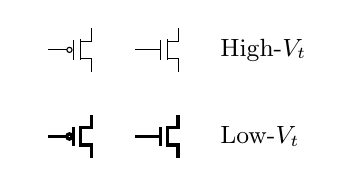
\begin{tikzpicture}[scale=.55,font=\small]
\mos{0}{3}{}{1}\mos{2}{3}{}{0}\node[right]at(3,3){High-$V_t$};
\begin{scope}[very thick]\mos{0}{1}{}{1}\mos{2}{1}{}{0}\end{scope}\node[right]at(3,1){Low-$V_t$};
\end{tikzpicture}\\\small Figure 1: (a) A CMOS circuit (b) High-/low-$V_t$ transistor symbols.\end{center}
\qheading{3. (20 points)} Consider a buffer chain shown in Fig. 2, used to drive a large capacitance $C_L$. The first-stage buffer is minimum size with input capacitance $C_i$. Each buffer has transistor width larger than the previous one by a factor $\beta$. Neglect parasitic capacitance.
\textbf{(a) (10 points)} What are the size ratio $\beta$ and number of stages $N$ such that the delay of the buffer chain is minimal?
\newpage
\begin{center}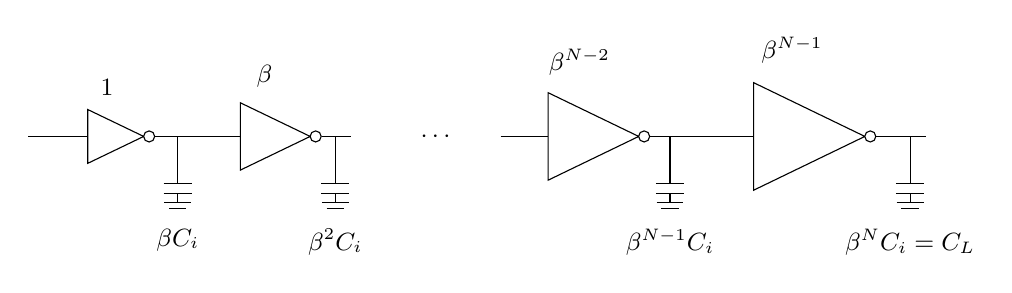
\begin{tikzpicture}[x=1cm,y=1cm,font=\small]
\node[not gate US,draw,minimum width=.8cm](a)at(0,1){};\node[not gate US,draw,minimum width=1cm](b)at(2,1){};
\node[not gate US,draw,minimum width=1.3cm](c)at(6,1){};\node[not gate US,draw,minimum width=1.6cm](d)at(8.7,1){};
\draw(-1,1)--(a.input);\draw(a.output)--(b.input);\draw(b.output)--(3.1,1);\node at(4.2,1){$\cdots$};\draw(5.0,1)--(c.input);\draw(c.output)--(d.input);\draw(d.output)--(10.4,1);
\foreach\x/\cap in {.9/\beta C_i,2.9/\beta^2C_i,7.15/\beta^{N-1}C_i,10.2/\beta^NC_i=C_L}{\draw(\x,1)--(\x,.4);\draw(\x-.18,.4)--(\x+.18,.4);\draw(\x-.18,.28)--(\x+.18,.28);\ground{\x}{.28}\node[below]at(\x,-.05){$\cap$};}
\node[above]at(0,1.4){1};\node[above]at(2,1.5){$\beta$};\node[above]at(6,1.65){$\beta^{N-2}$};\node[above]at(8.7,1.8){$\beta^{N-1}$};
\end{tikzpicture}\\\small Figure 2: A taper buffer for driving a large capacitance.\end{center}
\textbf{3(b). (10 points)} Calculate the power efficiency $\eta$, where $\eta=(P_T-P_L)/P_T$, when the optimized ratio is used to design the buffer chain. Here $P_T$ and $P_L$ denote total switching power of the buffer chain and load capacitance $C_L$, respectively.
\qheading{4. (10 points)} The figure in Fig. 3 depicts an inverter chain driving a capacitive load $C_L$. Every inverter has a minimum-size NMOS and the PMOS/NMOS ratio is $\alpha$. Let $\mu_n=2\mu_p$ and let the resistance and input capacitance of the minimum-size NMOS be $R$ and $C$. Derive $\alpha$ such that $T=6RC$ and the power consumption constituted by the first two inverters is minimal.
\begin{center}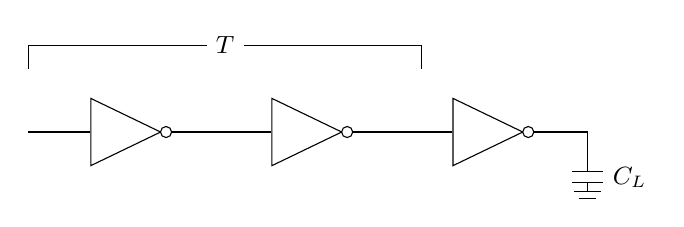
\begin{tikzpicture}[x=1cm,y=1cm,font=\small]
\node[not gate US,draw,minimum width=1cm](a)at(0,1){};\node[not gate US,draw,minimum width=1cm](b)at(2.3,1){};\node[not gate US,draw,minimum width=1cm](c)at(4.6,1){};
\draw(-1.1,1)--(a.input);\draw(a.output)--(b.input);\draw(b.output)--(c.input);\draw(c.output)--(6,1)--(6,.5);\draw(5.8,.5)--(6.2,.5);\draw(5.8,.36)--(6.2,.36);\ground{6}{.36}\node[right]at(6.2,.42){$C_L$};
\draw(-1.1,1.8)--(-1.1,2.1)--(3.9,2.1)--(3.9,1.8);\node[fill=white]at(1.4,2.1){$T$};
\end{tikzpicture}\\\small Figure 3: An inverter pair. (The printed figure contains three inverters; $T$ brackets the first two.)\end{center}
\qheading{5. (10\%)} Table 1 shows the truth table of a binary full adder, where $c_i,s$, and $c_o$ denote carry input, sum output, and carry out. Design a full adder using CMOS logic with PMOS and NMOS transistors.
\begin{center}\small Table 1: Truth table of a binary full adder.\\
\begin{tabular}{ccccc}\toprule$x$&$y$&$c_i$&$s$&$c_o$\\\midrule
0&0&0&0&0\\0&0&1&1&0\\0&1&0&1&0\\0&1&1&0&1\\
1&0&0&1&0\\1&0&1&0&1\\1&1&0&0&1\\1&1&1&1&1\\\bottomrule\end{tabular}\end{center}
\vfill\small Original footer: Li, EE, NCU; Spring 2008. All five questions and printed allocation marks are retained.\end{document}
